\setAuthor{}
\setRound{lõppvoor}
\setYear{2019}
\setNumber{G 6}
\setDifficulty{6}
\setTopic{TODO}

\prob{Lõks}
Kuulike massiga $m$ ja laenguga $q$ sisenes läbi väikse augu silindrisse, mida täidab teljesihiline homogeenne magnetväli induktsiooniga $B$. Sisenemishetkel oli kuulikese kiirus radiaalsihiline. Kuulike väljus silindrist sama augu kaudu peale kahte absoluutselt elastset põrget silindri seintega. Kui kaua viibis kuulike silindris? 
\vspace{-5pt}


\hint

\solu
\begin{wrapfigure}[7]{r}{0.41\textwidth}
  \vspace{-25pt}
  \begin{center}
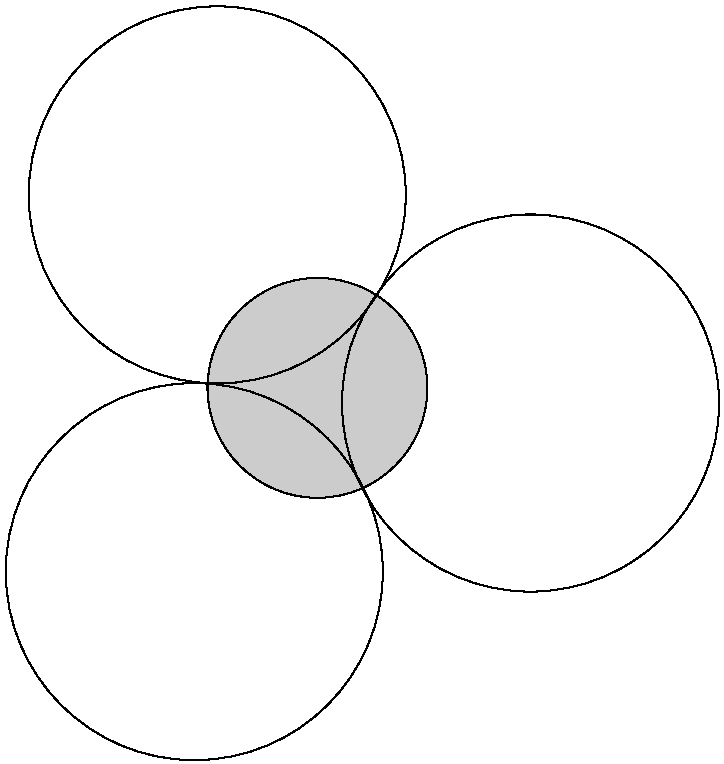
\includegraphics[scale=0.3]{2019-v3g-06-sol.pdf}
    % Pildi allikas Wikimedia Commons https://upload.wikimedia.org/wikipedia/commons/4/4f/Curling_stones.jpg
  \end{center}
  \vspace{-20pt}
\end{wrapfigure}

Kuulikese trajektoor silindris koosneb kolmest kaarejupist nii nagu näidatud joonisel. Nagu jooniselt näha, igale kaarejupile vastav kesknurk on 60 kraadi, seega trajektooride kesknurkade summa on pool täisringist, st kuulike veedab silindris pool tsüklotronperioodist  $t=T/2=\pi\frac m{qB}$.
\probend